\chapter{Basics}
\label{chap:basics}

This chapter is a brief introduction to hydropower. It presents the origin and quantification of hydro resource, and gives an overview of the conversion devices with a focus on run-of-the-river (ROR) power plants.

\section{Hydro resource}

\subsection{Characteristics}

On Earth, water is continuously moving in liquid, gaseous or solid form, in a process called the hydrologic cycle. Water evaporates, is transported by winds, falls out as rain or snow, gathers into streams and rivers, and flows into seas or lakes. All this movement provides an enormous opportunity to harness useful energy \cite{ucsusa}. Kinetic and potential energy of water can set turbines in motion, creating mechanical energy, which can then be turned into electric energy. The global technically exploitable hydropower potential is estimated at more than 16 400 TWh per year, around 19\% of which have been developed worldwide \cite{iea_hp_ess}.
 
\subsection{Runoff prediction}
 
Modelling runoff is a difficult task, as the model has to assess the interactions between river sources, relief, rainfall, local soil and vegetation type, as well as anthropogenic use. This can be done using GIS \cite{bayazit}, by assigning each cell with the precedent parameters. The water input in each cell (rainfall, water sources and runoff from other cells) is converted in runoff from the cell by subtracting the water lost by infiltration, evapotranspiration, or anthropogenic use, and the runoff direction is given by the slope, calculated using a digital elevation model \cite{heywood}. \newline
The waterGAP software, developed by the universities of Kassel and Frankfurt, uses this method to calculate flows and storages of water around the globe, as shown on figure \ref{waterGAP}.

\begin{figure}[H]
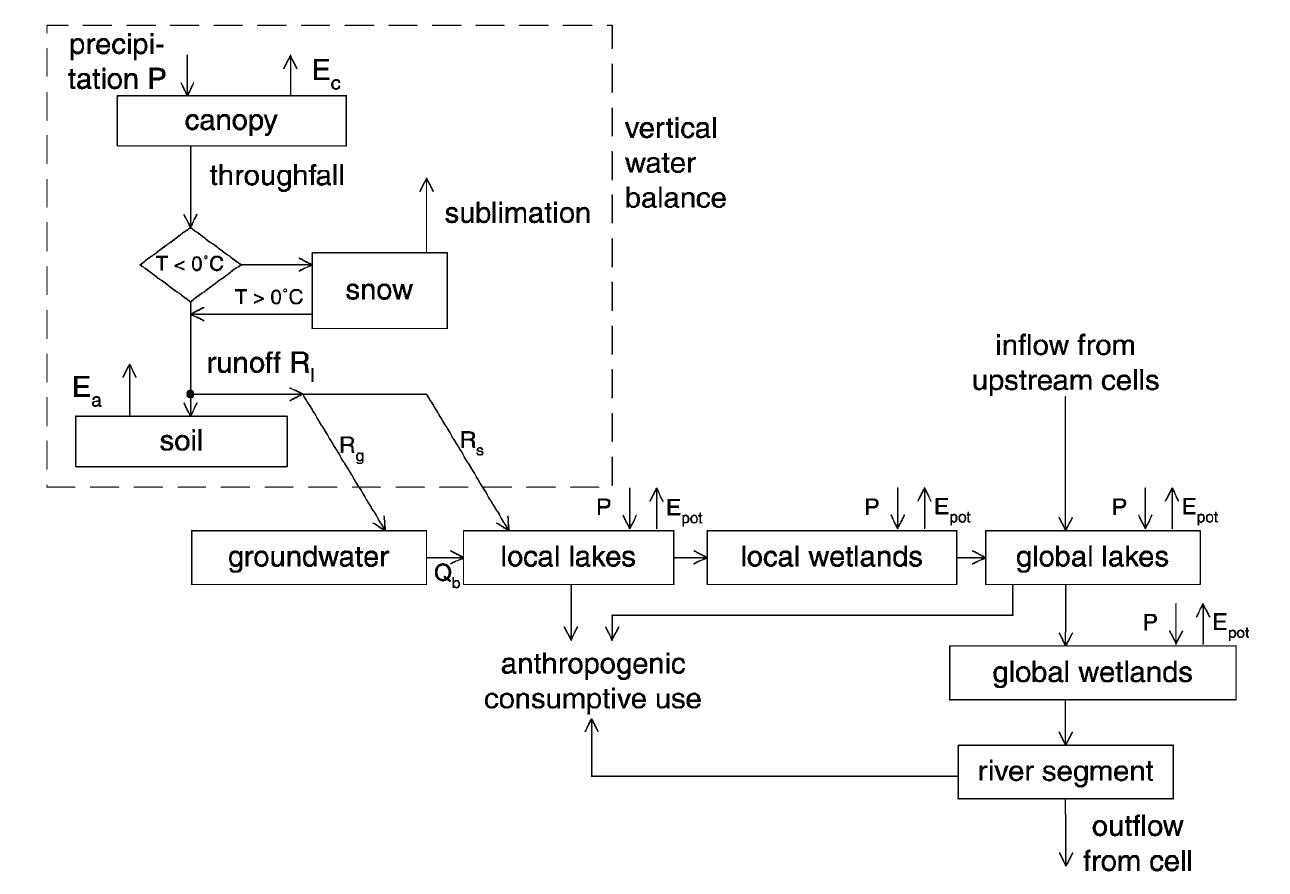
\includegraphics[width=15cm]{waterGAP.png}
\caption[Representation of a global hydrological from the WaterGAP software]{Representation of a global hydrological from the WaterGAP software \cite{doll}}
\centering
\label{waterGAP}
\end{figure}

 
\subsection{Measured runoff}
 
In order to study rivers, measurement stations have been installed and monitored for decades, dating back as far as 1816 for Germany. These stations measure the water level or the flow volume with a given timestep and the data is stored in databases. There are different ways to measure the water flow, such as propeller gauges, ultrasonic flow meter, or acoustic current profilers.In Germany, there are around 4300 stations measuring water flow or water level, operated by different stakeholders \cite{bafg_hyd}.
 
\section{Types of hydropower plants}

The main types of hydroelectrcity generating methods are conventional hydropower (dams), pumped storage plants, run-of-the-river plants and tide power stations.

\subsection{Conventional}

Conventional hydroelectricity, or reservoir hydroelectricity, comes from the potential energy of dammed water. In a conventional power plant, the turbine is powered by an inflow from one or several reservoirs. Its use is thereby largely independant from the temporal course of the river flowing into the reservoir \cite{vgb}.

\subsection{Pumped storage}

A pumped storage power plant is a reservoir plant, whose reservoir is completely or partially filled with pumped water. In general, the water is pumped from a lower reservoir, which can be the reservoir of another power plant or a natural water body. A distinction is made between pumped storage with or without natural inflow in the upper reservoir \cite{vgb}.

\subsection{Run-of-the-river}

Run-of-the-river hydropower plants are hydropower plants that uses the natural usable stream without delaying it \cite{vgb}. They do not accumulate water in a reservoir and are therefore dependant on the flow of the river.

\subsection{Others}

Other types of hydropower include devices converting energy from the tides or the waves.

\section{Theory of ROR power plants}
\subsection{Operating}
Quaschning \cite{quaschning} describes how a run-of-the-river power plant operates.Even though there is no reservoir accumulating the water upstream from the plant, run-of-the-river power plants need an altitude difference, called head, between the water surface before and after the plant. This can be achieved through a dam, a derivation of the water stream through a canal, or a lock \cite{tdi_petites_centrales}. The water is lead through a turbine (see figure \ref{schema_hpp}) that drives a electrical generator.
\begin{figure}[H]
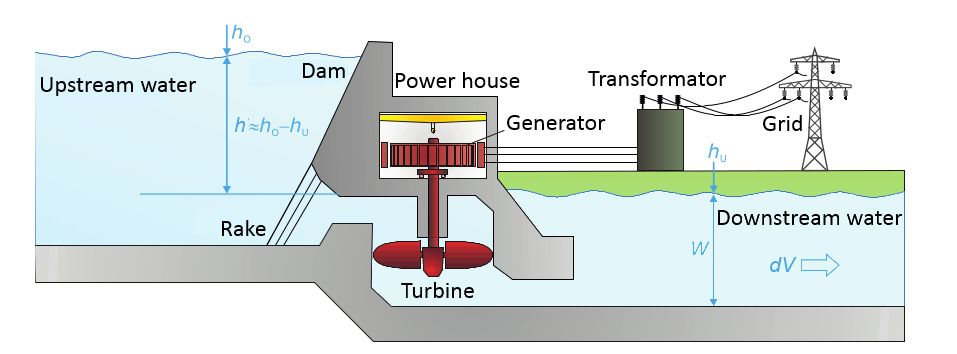
\includegraphics[width=15cm]{schema_hpp_en.png}
\caption[Schema of a run-of-the-river hydropower plant]{Schema of a run-of-the-river hydropower plant \cite{quaschning}}
\centering
\label{schema_hpp}
\end{figure}
\subsection{Output power}
A run-of-the-river power plant generates a power proportional to the water flow and the head, as seen in equation \ref{eq_power_1} \cite{quaschning}.
\begin{equation}
\label{eq_power_1} 
 P = \rho_\mathrm{water} \cdot g \cdot Q_\mathrm{turbine} \cdot H \cdot \eta_\mathrm{turbine} \cdot \eta_\mathrm{generator}
\end{equation}
With 
\begin{itemize}
\itemsep0em 
 \item $P$ \tabto{4cm} power produced by the generator \tabto{12cm} $[W]$
 \item $\rho_\mathrm{water}$ \tabto{4cm} density of water \tabto{12cm} $1000 \ kg/m^3$
 \item $g$ \tabto{4cm} acceleration of gravity \tabto{12cm} $9.81 \ m/s^2$
 \item $Q_\mathrm{turbine}$ \tabto{4cm} water flow through the turbine \tabto{12cm} $[m^3/s]$
 \item $H$ \tabto{4cm} head of water \tabto{12cm} $[m]$
 \item $\eta_\mathrm{turbine}$ \tabto{4cm} efficiency of the turbine
 \item $\eta_\mathrm{generator}$ \tabto{4cm} efficiency of the generator
\end{itemize}


The head of water is the altitude difference between the surface of the river before and after the turbine. For run-of-the-river hydropower plants, it is assumed that the water level before the turbine is kept constant by the dam, while the water level downstream can vary. This happens when the waterflow exceeds the capacity of the turbine and has to be deviated over the dam. With this assumption, the head of water is given by the equation \ref{eq_head} and the waterflow in the turbine by the equation \ref{eq_waterflow} \cite{quaschning}.
\begin{equation}
\label{eq_head} 
 H = H_\mathrm{n} +W_\mathrm{n}-W
\end{equation}
\begin{equation}
\label{eq_waterflow} 
 Q_\mathrm{turbine} = min(Q_\mathrm{n},Q)
\end{equation}
Where $H_\mathrm{n}$, $W_\mathrm{n}$ and $Q_\mathrm{n}$ are respectively the nominal head, water level downstream from the dam and water flow, and W and Q the real water level and water flow.
\newline
The  equation \ref{eq_power_1} becomes :
\begin{equation}
 \label{eq_power_2} 
 P = \rho_\mathrm{water} \cdot g \cdot min(Q_\mathrm{n},Q) \cdot (H_\mathrm{n} +W_\mathrm{n}-W) \cdot \eta_\mathrm{turbine} \cdot \eta_\mathrm{generator}
\end{equation}

\subsection{Types of turbines}

There are two families of water turbines : action turbines and reaction turbines. Action turbines use the kinetic energy of water, without any changes in pressure, while reaction turbines transform the potential energy of water into kinetic energy, decreasing the pressure. The main types of turbines for each family are \cite{quaschning} :
\begin{itemize}
 \item Action turbines
 \begin{itemize}
  \item Pelton turbine
  \item Turgo turbine
  \item Ossberger turbine or cross-flow turbines
 \end{itemize}
 \item Reaction turbines
 \begin{itemize}
  \item Kaplan turbines
  \item Bulb or tubular turbines
  \item Francis turbines
 \end{itemize}
\end{itemize}


\subsection{Turbine efficiency}

The efficiency of the turbine depends on the type of turbine and on the part-load range \cite{quaschning}\cite{pacer}. There are four types of turbines used for run-of-the-river plants : Pelton, Francis, Kaplan and crossflow. These turbines have optimal performances over ranges of water flow and hydraulic head, and their application areas can be plotted on a characterisitc diagramm, as in figure \ref{charac_diag}. 

\begin{figure}[H]
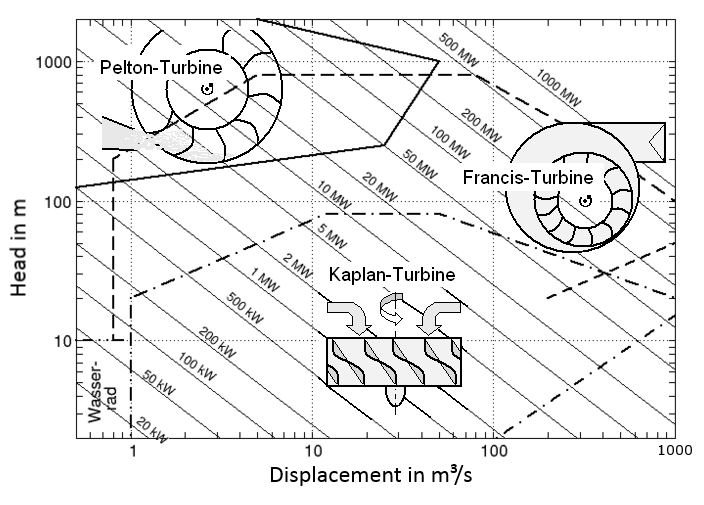
\includegraphics[width=14cm]{charac_diag_en.png}
\caption[Characteristic diagramm for several types of water turbines]{Characteristic diagramm for several types of water turbines \cite{wiki_WK}}
\centering
\label{charac_diag}
\end{figure}

Figure \ref{efficiency_turb} give the efficiency curves of different turbine types depending on the part load. These efficiencies can be approximated by the empiric function given in equation \ref{eq_eff} with the parameters given in table \ref{eff_param} \cite{quaschning}. In this equation, $Q_\mathrm{min}$ is the minimal water flow to start the turbine, $Q_\mathrm{n}$ is the nominal waterflow of the turbine and $q=\frac{Q-Q_\mathrm{min}}{Q_\mathrm{n}}$.

\begin{equation}
 \label{eq_eff}
\eta_\mathrm{T}= \left\{
    \begin{array}{ll}
	0 & \mbox{for } Q \leq Q_\mathrm{min}\\
        \frac{q}{a_\mathrm{1}+a_\mathrm{2} \cdot q + a_\mathrm{3} \cdot q^2} & \mbox{for } Q_\mathrm{min}<Q<Q_\mathrm{n} \\
        \eta_\mathrm{T,n} & \mbox{for } Q \geq Q_\mathrm{n}
    \end{array}
\right.
\end{equation}


\begin{figure}[H]
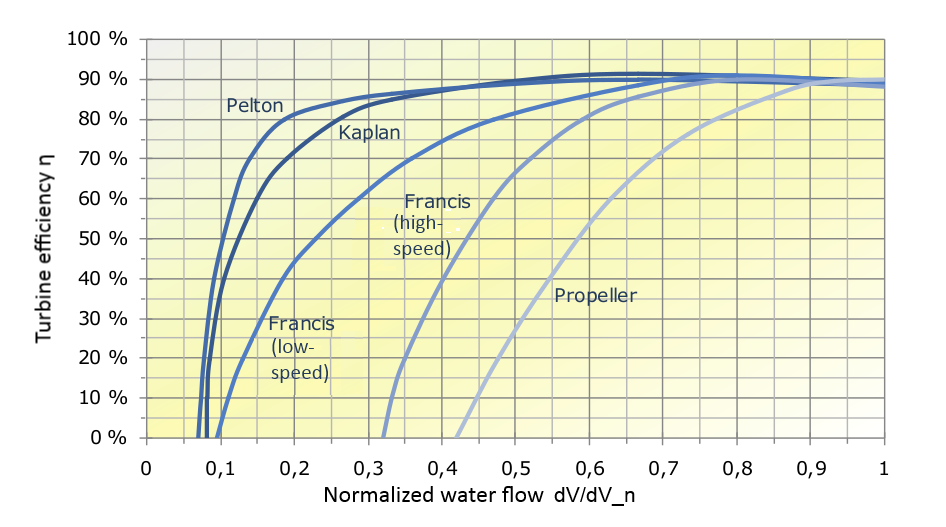
\includegraphics[width=15cm]{efficiency_turb_en.png}
\caption[Efficiency of different types of turbines depending on the part load ratio]{Efficiency of different types of turbines depending on the part load ratio (water flow / nominal water flow) \cite{raa89}}
\centering
\label{efficiency_turb}
\end{figure}


\begin{table}
 \caption[Parameters to calculate the turbine efficiency]{Parameters to calculate the turbine efficiency \cite{quaschning}}
 \label{eff_param}
 \centering
 \begin{tabular}{|c|c|c|c|c|c|}
  \cline{2-6}
  \multicolumn{1}{c|}{}&$Q_\mathrm{min} / Q\mathrm{n}$ & $\eta_\mathrm{T,n}$& $a_\mathrm{1}$ & $a_\mathrm{2}$&$a_\mathrm{3}$ \\ 
  \hline
  Kaplan & 0.081& 0.895& 0.045 &0.965& 0.1 \\
  Pelton & 0.07& 0.885& 0.03& 0.99& 0.1\\
  Francis &0.095 &0.89 &0.18 &0.63 &0.31 \\
  Propeller &0.42 &0.9 &0.25 &0.28 &0.69\\
  \hline
 \end{tabular}
\end{table}

\subsection{Generator efficiency}

The efficiency factor of the generator depends on its power and on the part-load range \cite{pacer}. The swiss ``Bundesamt für Konjunkturfragen'' gives the values given in table \ref{eta_gen}.

\begin{table}
 \caption[Generator efficiency in full load and part load]{Generator efficiency in full load (left) and part load (right) \cite{pacer}}
 \label{eta_gen}
 \begin{tabular}{|C{3cm}|C{3cm}| C{1cm} |C{3cm}|C{3cm}|}
  \cline{1-2} \cline{4-5}
  $P_\mathrm{el} [kW]$ & $\eta_\mathrm{g,max}$  && $P_\mathrm{el}/P_\mathrm{el, max}$ & $\eta_\mathrm{g}/\eta_\mathrm{g,max}$ \\ 
  \cline{1-2} \cline{4-5}
  1 to 5 & 80\% to 85\% && 
  \multirow{4}{*}{\begin{tabular}{c}>50\%\\25\% \\10\% \\\end{tabular}}& 
  \multirow{4}{*}{\begin{tabular}{c}100\% \\95\% \\85\% \\\end{tabular}}\\
  5 to 20 & 85\% to 90\% &&& \\
  20 to 100 & 90\% to 95\% &&&\\ 
  More than 100 & 95\% &&&\\ 
  \cline{1-2} \cline{4-5}
\end{tabular}
\end{table}

It is estimated that among the 6500 to 7500 hydropower plants in Germany, only 406 have a nominal power above 1MW \cite{uba_wasserkraft}. Out of 7500 run-of-the-river hydropower plants in the OpenEnergy Database, 5600 have a capacity under 100kW (see figure \ref{oedb_capa} in section \ref{hpp_register}).  However, the plants under 1MW account for a small part of the total installed power (see figure \ref{uba_hpp}). For that reason, the generator efficiency has been approximated to 95\% for all power plants is this work.

\begin{figure}[H]
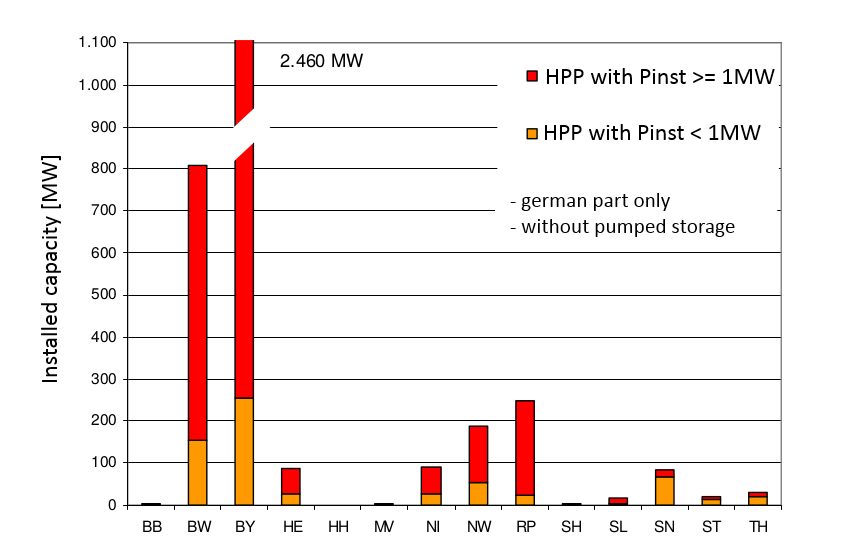
\includegraphics[width=15cm]{uba_hpp_en.png}
\caption[Installed power pro Bundesland for plants over and under 1MW]{Installed power pro Bundesland for plants over and under 1MW \cite{uba_wasserkraft}}
\centering
\label{uba_hpp}
\end{figure}
